\scanpage{19}
de Kostant. On a donc des morphismes $f\handwritten{\unsure{\mathrel{\mapstochar\relbar}|\mapsto}}f\handwritten{\circ}i_o$ et $f\handwritten{\mapsto}f(u_o)$ de $\operatorname{Dyn}_c$ dans $\operatorname{ST}_c$ resp. $\operatorname{Un}_c$. D'autre part, Deligne nous fournit $\operatorname{Un}_c\handwritten{\to\underline{\varnothing}}_c$, et celui-ci peut aussi être défini par la commutativité du diagramme \handwritten{d'esp. homogènes}
\diagram{%
\begin{tikzcd}[ampersand replacement=\&]
\operatorname{ST}_c\handwritten{\simeq}(\operatorname{CL})_{c'} \handwritten{\arrow[d]} \& \operatorname{Dyn}_c \handwritten{\arrow[l]} \handwritten{\arrow[d]} \\
\handwritten{\underline{\varnothing}}_c\handwritten{\simeq}\operatorname{Par}_{c'} \& \operatorname{Un}_c\mathpunct{.} \handwritten{\arrow[l]}
\end{tikzcd}\qquad
\handwritten{\begin{tikzcd}[ampersand replacement=\&,column sep=small,row sep=small]
L \arrow[d] \&
{\vcenter{\hbox{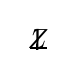
\begin{tikzpicture}[x=1em,y=1em,baseline=0pt]
\node[inner sep=0pt] at (.45,.45) {$\unsure{Z}$};
% The central overprint is retained without assigning an order to its strokes.
\draw[line width=.8pt] (.43,.82)--(.42,.06);
\draw[line width=.7pt] (.15,.11)--(.77,.11);
\end{tikzpicture}}}}_{\unsure{o|0}} \arrow[l] \arrow[d] \\
P \& \unsure{\mathfrak{z}|z|Z}(\unsure{\mathbin{.}}e) \arrow[l]
\end{tikzcd}}}

Pour qu'il existe un point rationnel de \deleted{$\operatorname{Dyn}_c$, ou ce qui revient au même} $\handwritten{\underline{\varnothing}}_c\handwritten{\simeq}\operatorname{Par}_{c'}$, il faut (et suffit) qu'il en existe un de $\operatorname{Dyn}_c$ \deleted{i.e. que $G$ soit quasi-déployé\unsure{;}}\inserted{\handwritten{(i.e.\unsure{,,|,} si $Z_o=e$, que $G$ est quasi-déployé)}}: en effet, $P$ étant choisi, \deleted{\unsure{les|des} $i$}%
% A separate cancellation x follows the overprinted group; no underlying letter is identifiable.

\begin{tikzpicture}[baseline=(cancelone.base)]\node[inner sep=0pt] (cancelone) {\texttt{x}};\end{tikzpicture}
on peut en choisir un \deleted{point rationnel}%
% The final cancellation x extends beyond the readable word.

\begin{tikzpicture}[baseline=(canceltwo.base)]\node[inner sep=0pt] (canceltwo) {\texttt{x}};\end{tikzpicture}
sous-groupe de Lévi
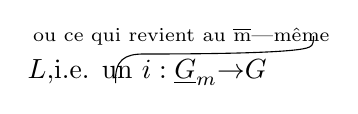
\begin{tikzpicture}[baseline=(levi.base),x=1em,y=1em]
\node[anchor=base west,inner sep=0pt] (levi) at (0,0) {$L$,\deleted{i.e}. un $i:\underline{G}_m\handwritten{\to}G$};
\node[anchor=base west,inner sep=0pt] at (.2,1.35) {\scriptsize\inserted{\handwritten{ou ce qui revient au \unsure{$\overline{\mathrm{m}}$|même}}}};
\draw[line width=.4pt] (3.2,-.15) .. controls (3.15,.7) and (3.55,.9) .. (4.2,.9) .. controls (7,.9) and (9.8,.95) .. (10.2,1.15) .. controls (10.35,1.2) and (10.35,1.4) .. (10.35,1.55);
\end{tikzpicture}
dans la classe $c$,définissant $P$, et alors les $u=\exp(e)$ qui \deleted{aux} s'adaptent à $i$ forment un ouvert dense de $\handwritten{\unsure{\mathfrak{g}|\mathscr{G}}(2)}$, qui \deleted{est donc non vide} a donc un point rationnel. On voit donc que pour certaines classes de paraboliques (qu'on pourrait appeler les paraboliques de
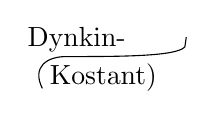
\begin{tikzpicture}[baseline=(kostant.base),x=1em,y=1em]
\node[anchor=base west,inner sep=0pt] (kostant) at (0,0) {Kostant\unsure{)}};
\node[anchor=base west,inner sep=0pt] at (-.8,1.35) {\inserted{Dynkin-}};
\draw[line width=.4pt] (-.25,-.15) .. controls (-.65,.65) and (-.05,1.0) .. (.6,1.0) .. controls (2.5,1.0) and (4.6,1.0) .. (4.9,1.35) -- (4.95,1.7);
\end{tikzpicture}
l'existence d'un parabolique de cette classe rationnel sur $k$ implique déjà que $G$ est quasi-déployé. (NB Quand $G$ n'est pas une forme intérieure, il faut faire attention cependant de vérifier d'abord que la classe $c'$ de $P$ provient bien d'un $c$ de Dynkin \uline{invariant par} $\handwritten{\Gamma}$, et il n'est pas clair que cette propriété
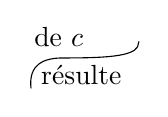
\begin{tikzpicture}[baseline=(resulte.base),x=1em,y=1em]
\node[anchor=base west,inner sep=0pt] (resulte) at (0,0) {résulte};
\node[anchor=base west,inner sep=0pt] at (-.25,1.35) {\inserted{de $c$}};
\draw[line width=.4pt] (-.35,-.15) .. controls (-.45,.75) and (.15,.95) .. (.8,.95) .. controls (2.3,.95) and (3.3,1.0) .. (3.5,1.35) -- (3.55,1.55);
\end{tikzpicture}
du fait que $c'$ est invariant\unsure{e|è} par $\handwritten{\Gamma}$, faute de savoir si $c\handwritten{\mapsto}c'$ est injectif sur les classes de Dynkin). \handwritten{(}On notera aussi que l'argument donné \deleted{p}marche également sur un anneau semi-local (de car. nulle jusqu'à nouvel ordre).\handwritten{)}
% margin note slanted upwards to the right; source line division retained
\margin{\handwritten{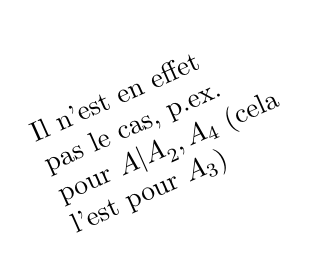
\begin{tikzpicture}
\node[anchor=south west,rotate=24,align=left,inner sep=0pt] at (0,0) {Il n'est en effet\\pas le cas, p.ex.\\pour $\unsure{A|\mathbb{A}}_2,A_4$ (cela\\l'est pour $A_3$)};
\end{tikzpicture}}}
Ceci montre l'intérêt, pour des questions arithmétiques, de déterminer exactement les
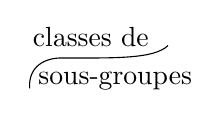
\begin{tikzpicture}[baseline=(sousgroupes.base),x=1em,y=1em]
\node[anchor=base west,inner sep=0pt] (sousgroupes) at (0,0) {sous-groupes};
\node[anchor=base west,inner sep=0pt] at (-.2,1.35) {\inserted{classes \handwritten{de}}};
\draw[line width=.4pt] (-.3,-.15) .. controls (-.35,.65) and (.25,.95) .. (.85,.95) .. controls (2.7,.95) and (4.2,.9) .. (4.7,1.4);
\end{tikzpicture}
parab\handwritten{\unsure{\begin{tikzpicture}[baseline=0pt,x=1em,y=1em]\draw[line width=.6pt] (0,0)--(.85,.22);\end{tikzpicture}}}oliques de Dynkin-Kostant des divers groupes simples, et de voir si\handwritten{\unsure{:|``}} leur stabilisateur dans $\operatorname{Autext}(G_o)$ est le même que celui des $c$ de Dynkin correspondants, et pas str. plus grand.

On notera cependant que si une filtration du foncteur \deleted{fib} oubli peut être définie par un élément unipotent, la classe de conjugaison de ce der%
% The source ends here with the continuation hyphen in der-; the word is left open for the next page.
% archive sheet number: 18
